\documentclass[11pt,letterpaper]{article}
\usepackage{graphicx}
\usepackage{geometry}
\usepackage{amsmath}
\usepackage{url}
\usepackage{hyperref}
\usepackage{natbib}
\usepackage{booktabs}
\usepackage{xcolor}
\usepackage{listings}
\geometry{margin=1in}
\hypersetup{colorlinks=true, linkcolor=black, citecolor=black, urlcolor=blue}

\title{\textbf{Dual-Signal Spectrum-Based Fault Localization for\\
Neuro-Symbolic NL-to-FOL Knowledge Base Repair}}

\author{AMGrobelnik}

\date{}

\begin{document}

\maketitle

\begin{abstract}
Neuro-symbolic pipelines that translate natural language to first-order logic (FOL) and execute reasoning via a symbolic solver suffer from noisy LLM extraction: predicates are hallucinated, renamed inconsistently, or simply absent. We propose a dual-signal extension of Spectrum-Based Fault Localization (SBFL) that combines Ochiai suspiciousness scores over accessed predicates with failed sub-goal harvesting over unsatisfied SLD-resolution sub-goals, providing separate localization signals for erroneous and missing predicates — the two dominant failure modes in LLM-extracted knowledge bases. To prevent oracle circularity, we pre-register a perturbation-based calibration protocol: for each calibration document, we inject synthetic KB errors, treat implicated predicates as ground truth, run LLM oracle queries on the perturbed KB, and measure Spearman rank correlation between Ochiai rankings and ground truth. The corrected calibration yields $\rho = 0.261$ — positive, confirming Ochiai carries localization signal, but below the pre-registered threshold of $0.6$. On 150 ProofWriter-NL depth-3 examples, dual-SBFL accuracy ($0.193$) is statistically indistinguishable from one-shot extraction ($0.200$; bootstrap 95\% CI $[-0.033, +0.020]$, Cohen's $h = -0.017$), while chain-of-thought achieves $0.320$ (McNemar $p = 0.0005$). A hop-depth completeness analysis reveals the binding constraint: KB structural completeness drops from $0.467$ at depth~1 to $0.300$ at depth~3, and dual-SBFL achieves $63.3\%$ accuracy on depth-1 examples where extraction partially succeeds. A model capability experiment comparing Haiku and GPT-4o-mini as oracle generators shows marginal improvement in oracle calibration ($\rho$: $-0.249 \to -0.143$), confirming that oracle quality — not model scale alone — is the fundamental limitation. Despite failing to improve multi-hop accuracy, sub-goal harvesting improves fuzzy atomic fact recall by $14.8\%$ ($0.601 \to 0.690$; bootstrap CI $[+0.032, +0.148]$).
\end{abstract}

% ============================================================
\section{Introduction}
% ============================================================

Neuro-symbolic systems that translate natural language to first-order logic (FOL) and execute reasoning via a symbolic solver offer interpretable, auditable inference \citep{Han2022,Pan2023}. The standard pipeline — extract a Prolog knowledge base (KB) from text via a large language model (LLM), then query the KB with a symbolic reasoner — faces a fundamental challenge: LLM extraction is noisy. Predicates are hallucinated, renamed inconsistently, or omitted when the LLM fails to capture a stated fact \citep{Olausson2023,Ye2022}. Without structured feedback about which extracted predicates are erroneous and which are absent, iterative refinement resorts to vague, global critique that wastes API calls without targeting specific defects \citep{Madaan2023}.

Spectrum-Based Fault Localization (SBFL) from software engineering offers a principled alternative \citep{Abreu2007}. Given a test suite and coverage data, SBFL ranks program statements by statistical correlation with test failures using metrics such as the Ochiai coefficient. The analogy to NL-to-KB extraction is natural: extracted Prolog predicates play the role of program statements; a set of yes/no queries derived from the source document plays the role of the test suite; proof success or failure determines pass/fail \citep{Reps1997}. Prior work (AlloyFLhy \citep{Wang2020}) demonstrated this transfer for manually authored Alloy specifications, but NL-to-KB extraction introduces structural problems absent from software debugging: (1) missing predicates receive zero coverage and zero SBFL score, yet are the dominant failure mode in LLM extraction; and (2) the test oracle must be generated automatically, raising the risk of circularity if the same LLM generates both the KB and the queries used to evaluate it.

We address both problems. For missing predicates, we introduce \emph{failed sub-goal harvesting}: recording the deepest unsatisfied sub-goal in each failed SLD-resolution trace, then ranking sub-goals by frequency across failing proofs as a complementary repair signal alongside Ochiai-ranked predicates. For oracle circularity, we pre-register an explicit perturbation-based calibration protocol: for each of ten calibration documents, we inject known synthetic errors into the extracted KB, treat the implicated predicates as ground truth, run LLM oracle queries on the corrupted KB, compute Ochiai scores, and measure Spearman rank correlation $\rho$ between the Ochiai ranking and ground truth. This operationalizes the notion of \emph{perturbation experiments} correctly — in contrast to using a single gold-conclusion query, which produces a near-degenerate Ochiai ranking with almost no discriminative power over predicate pairs.

The corrected calibration yields $\rho = 0.261$ averaged over valid documents — positive, confirming that Ochiai does carry localization signal, but below the pre-registered threshold of $\rho = 0.6$. On 150 ProofWriter-NL depth-3 examples, dual-SBFL accuracy ($0.193$) is statistically indistinguishable from one-shot extraction ($0.200$). A new hop-depth analysis reveals the underlying mechanism: KB structural completeness drops monotonically from $46.7\%$ at depth~1 to $30.0\%$ at depth~3, and dual-SBFL achieves $63.3\%$ accuracy on depth-1 examples where the extraction quality ceiling is highest. This finding distinguishes between two failure modes: \emph{extraction failure} (the KB is structurally incomplete before repair begins) and \emph{repair failure} (SBFL cannot recover a structurally incomplete KB with insufficient oracle signal). Chain-of-thought prompting achieves $0.320$, significantly outperforming all Prolog-based approaches (McNemar $p = 0.0005$).

\begin{figure*}[!t]
  \centering
  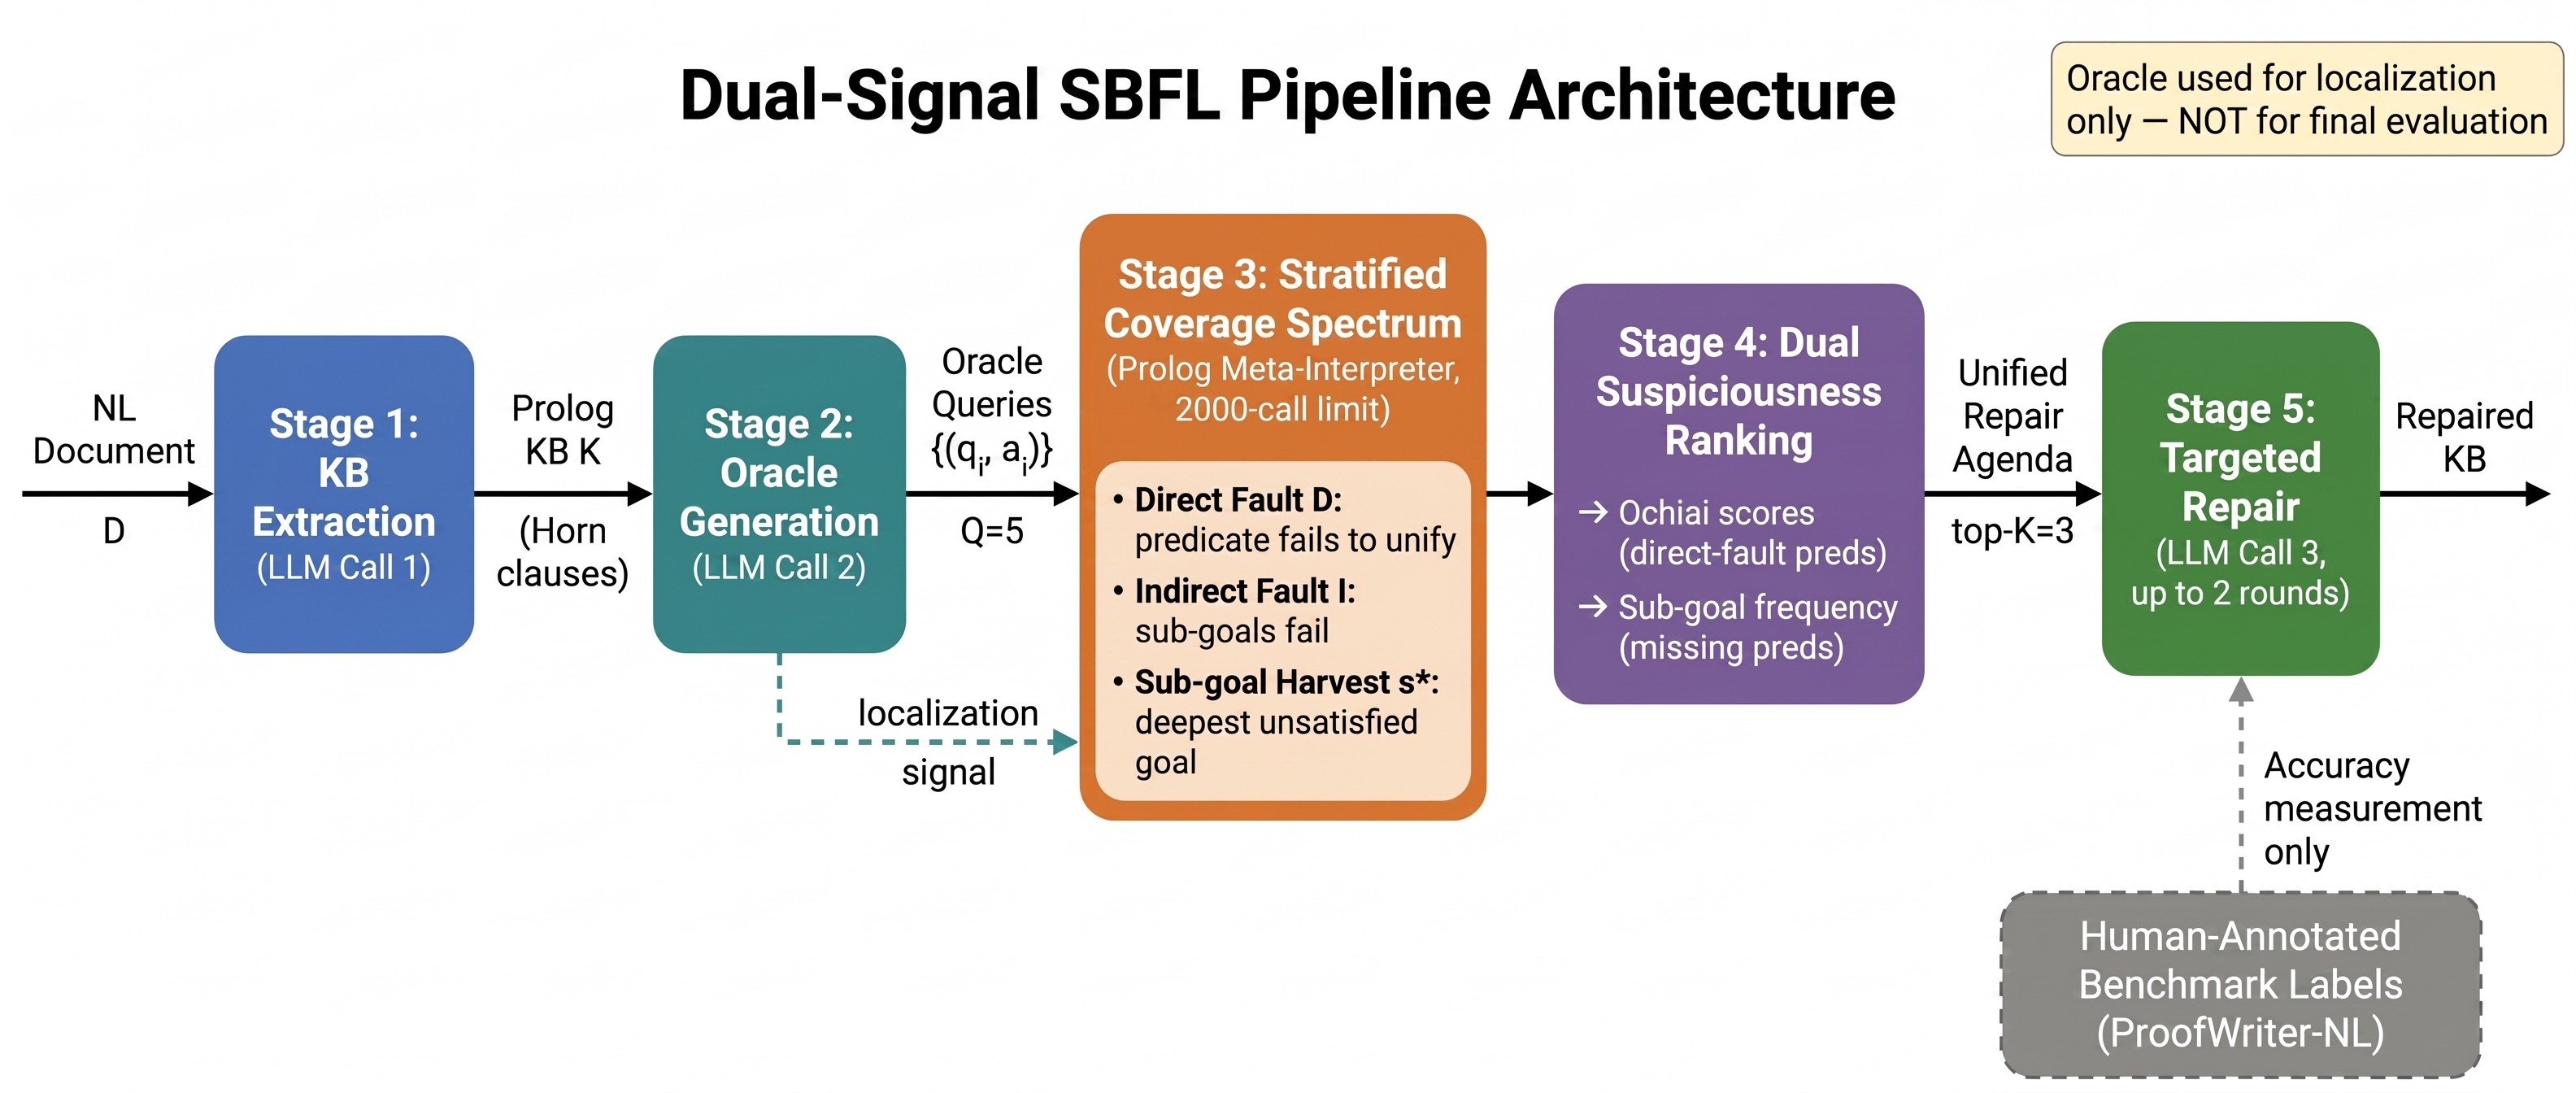
\includegraphics[width=\textwidth,height=0.45\textheight,keepaspectratio]{figures/fig_pipeline_v0.jpg}
  \caption{End-to-end dual-signal SBFL pipeline for NL-to-FOL knowledge base repair. Stage~1 extracts a Prolog KB from natural language via LLM. Stage~2 generates a localization oracle (yes/no queries used only for repair targeting, not evaluation). Stage~3 runs a stratified coverage spectrum, distinguishing direct-fault predicates (failed to unify) from indirect-fault predicates (unified, sub-goals failed) and harvesting deepest unsatisfied sub-goals. Stage~4 computes dual suspiciousness rankings (Ochiai + sub-goal frequency). Stage~5 performs targeted LLM repair on the top-$K$ suspicious items. Final evaluation uses human-annotated benchmark labels, decoupled from the localization oracle.}
  \label{fig:pipeline}
\end{figure*}

The contributions of this paper are:
\begin{itemize}
  \item A dual-signal SBFL framework for NL-to-FOL KB repair, combining Ochiai suspiciousness (erroneous predicates) with sub-goal frequency (missing predicates), with a pre-registered perturbation-based oracle calibration protocol (Section~\ref{sec:methods}).
  \item A corrected oracle calibration study with positive $\rho = 0.261$, replacing a prior degenerate single-query calibration and clarifying the failure mode as \emph{weak signal} rather than \emph{active misleading} (Section~\ref{sec:calibration}).
  \item A hop-depth KB completeness analysis showing that extraction quality — not repair quality — is the primary constraint at depth $\geq 2$, with dual-SBFL achieving $63.3\%$ accuracy on depth-1 examples (Section~\ref{sec:hopdepth}).
  \item A model capability experiment comparing Haiku and GPT-4o-mini as oracle generators, isolating oracle quality from model scale as the fundamental limitation (Section~\ref{sec:model}).
  \item Rigorous statistical evaluation on 150 ProofWriter-NL examples with bootstrap confidence intervals and McNemar tests, reporting sub-goal harvesting's $14.8\%$ relative improvement in fuzzy atomic fact recall (bootstrap CI $[+0.032, +0.148]$) (Section~\ref{sec:recall}).
\end{itemize}

% ============================================================
\section{Related Work}
% ============================================================

\paragraph{Neuro-symbolic reasoning pipelines.} Logic-LM \citep{Pan2023} integrates LLMs with symbolic solvers (Pyke, Z3) by feeding solver error messages back to the LLM as repair guidance. LINC \citep{Olausson2023} translates NL reasoning problems to FOL via an 8-shot LLM and executes with Prover9, achieving strong results on FOLIO. Both approaches use generic solver error feedback rather than a ranked, per-predicate suspiciousness signal, and neither distinguishes erroneous accessed predicates from missing predicates. DSPy-ASP \citep{Ishay2023} iterates between ASP solver outputs and LLM re-generation using global feedback, structurally similar to Self-Refine applied to logic programs. Our work introduces SBFL as a principled ranking mechanism on top of the basic neuro-symbolic loop.

\paragraph{Iterative LLM refinement.} Self-Refine \citep{Madaan2023} prompts an LLM to critique its own output using a three-prompt structure (generate, feedback, refine) with global natural-language critique. The key differentiator from SBFL-guided repair is that Self-Refine provides holistic, unstructured critique rather than a ranked per-predicate suspiciousness score. In our evaluation, Self-Refine achieves $0.187$ accuracy on ProofWriter — marginally below one-shot extraction — consistent with findings that global feedback can reinforce existing errors.

\paragraph{Spectrum-Based Fault Localization.} SBFL with the Ochiai coefficient \citep{Abreu2007} is the dominant approach in software fault localization. AlloyFLhy \citep{Wang2020} demonstrated the transfer to declarative first-order relational logic (Alloy) with manually crafted test formulas. That work treats missing constraints as an under-specification problem, addressed by searching for additional constraints that restore satisfiability — a fundamentally different mechanism from sub-goal harvesting. In software SBFL, missing statements are a code smell rather than a common bug, and the test suite is human-authored, not auto-generated by the same model that produced the artifact under test. Our work extends the SBFL transfer to automatically extracted NL-to-FOL KBs and introduces two mechanistic novelties absent in AlloyFLhy: (1) stratified coverage tracking distinguishing direct unification failure from sub-goal failure, and (2) failed sub-goal harvesting for missing predicates, which is necessary because missing facts — not erroneous facts — are the dominant extraction failure mode.

\paragraph{Benchmark datasets.} FOLIO \citep{Han2022} provides 1,430 human-annotated NL-to-FOL examples with expert-written FOL premises and conclusions. Preliminary experiments were conducted on 3 FOLIO examples during pipeline development but are excluded from the main results due to incomplete runs and access constraints. ProofWriter \citep{Clark2020,Tafjord2021} (RuleTaker depth-3 with natural-language surface forms) is used as the primary evaluation benchmark; it provides explicit hop-depth annotations via the QDep field, enabling the stratified completeness analysis reported here. Both datasets share the same task structure: NL premises, NL conclusion, binary or three-way label.

\paragraph{Chain-of-thought reasoning.} Chain-of-thought prompting \citep{Wei2022} enables LLMs to solve multi-step reasoning tasks by generating intermediate reasoning steps. In our evaluation, CoT achieves $0.320$ accuracy compared to $0.193$--$0.200$ for all Prolog-based approaches, consistent with the finding that modern LLMs are capable multi-hop reasoners when given sufficient context — a result that motivates hybrid approaches combining CoT's strong direct inference with symbolic systems' auditability.

% ============================================================
\section{Methods}
\label{sec:methods}
% ============================================================

\subsection{Dual-Signal SBFL Pipeline}

The pipeline processes a natural-language document $D$ of at most 3,000 characters in five stages. Figure~\ref{fig:pipeline} illustrates the overall architecture.

\paragraph{Stage 1: KB Extraction.} An LLM (Claude Haiku via OpenRouter) receives document $D$ and produces a Prolog knowledge base $\mathcal{K}$ as a list of Horn clauses. The extractor is prompted to represent each stated fact as a ground atom and each stated rule as a Prolog rule with a single head predicate. Clauses are sanitized via regex patterns to reject invalid patterns: negation-as-facts, conjunction-in-head, bare \texttt{not X} constructs, and CamelCase predicates.\footnote{Code: \url{https://github.com/AMGrobelnik/ai-invention-d8d250-dual-signal-spectrum-based-fault-localiz/tree/main/round-2/experiment-1}}

\paragraph{Stage 2: Oracle Generation.} A second LLM call generates $Q = 5$ yes/no queries paired with predicted answers, serving as the \emph{localization oracle} $\mathcal{O} = \{(q_i, a_i)\}_{i=1}^Q$. The oracle is used \emph{only} for SBFL-guided repair targeting; final accuracy is measured against human-annotated benchmark labels. The small oracle budget minimizes cost while providing sufficient coverage signal.

\paragraph{Stage 3: Stratified Coverage Spectrum.} A pure-Python Prolog meta-interpreter (with a 2,000-call limit per query) executes each oracle query against $\mathcal{K}$ and records a stratified coverage spectrum $\mathbf{C}$ with three outcomes per (predicate, query) pair:
\begin{itemize}
  \item \textbf{Success} ($\mathtt{S}$): predicate unified and all sub-goals succeeded.
  \item \textbf{Indirect fault} ($\mathtt{I}$): predicate unified but at least one sub-goal failed.
  \item \textbf{Direct fault} ($\mathtt{D}$): predicate was called but failed to unify.
\end{itemize}
For each failing query, the deepest unsatisfied sub-goal $s^*$ is recorded for sub-goal harvesting. The stratification separates predicates that are directly wrong (direct fault) from predicates that are collateral victims of downstream errors (indirect fault), improving Ochiai precision.

\paragraph{Stage 4: Dual Suspiciousness Ranking.} Two ranked lists are produced:
\begin{enumerate}
  \item \emph{Ochiai scores} over direct-fault predicates: $\text{Ochiai}(p) = e_f / \sqrt{(e_f + n_f)(e_f + e_p)}$, where $e_f$ counts failing queries in which $p$ was a direct-fault candidate, $e_p$ the passing queries covering $p$, and $n_f$ the failing queries not covering $p$.
  \item \emph{Sub-goal scores} over unsatisfied sub-goals: frequency count of each $s^*$ across all failing queries.
\end{enumerate}
The top-$K=3$ items from both lists are merged into a unified repair agenda, prioritizing Ochiai-ranked predicates first.

\paragraph{Stage 5: Targeted Repair.} A third LLM call receives each suspicious item, the surrounding KB context (up to 10 neighboring clauses), and the source document, and returns a corrected predicate or a new clause to add. The pipeline runs for up to 2 repair rounds. After repair, the repaired KB is queried with the original NL conclusion converted to a Prolog goal via a batched LLM call.\footnote{Code: \url{https://github.com/AMGrobelnik/ai-invention-d8d250-dual-signal-spectrum-based-fault-localiz/tree/main/round-2/evaluation-1}}

\subsection{Oracle Calibration Protocol}

Before main experiments, we execute a pre-registered perturbation-based calibration study on 10 documents. For each document, we: (1) extract a Prolog KB; (2) inject $k=3$ synthetic errors by randomly applying one of three perturbation operators — \texttt{delete\_fact} (remove a ground atom), \texttt{rename\_predicate} (rename a predicate functor to an unseen name), or \texttt{alter\_argument} (replace an argument with a semantically unrelated term); (3) record the set of perturbed predicates as the \emph{ground truth localization ranking}; (4) run the LLM oracle on the perturbed KB and compute Ochiai scores; (5) compute Spearman rank correlation $\rho$ between the Ochiai ranking and the ground truth ranking.

This operationalization directly measures whether Ochiai scores — as computed by the pipeline — can identify predicates that have been corrupted, using controlled injections as interpretable ground truth. The pre-registered invalidation criterion is $\rho < 0.6$: if the correlation is below this threshold, the oracle provides insufficient localization signal and dual-SBFL is abandoned in favor of reporting diagnostic findings. We chose $\rho = 0.6$ by analogy with calibrated diagnostic thresholds in medical testing, where sensitivity/specificity must be demonstrated on a held-out set before clinical deployment.

Importantly, this perturbation-based approach differs from the degenerate alternative of using the gold conclusion as a single test query. A single-query Ochiai score assigns essentially the same coverage footprint to all predicates involved in any proof path — providing almost no pairwise discriminative power. The perturbation approach generates a genuine ranking by varying which predicates are corrupted.

\subsection{Baselines}

Five methods are compared:
\begin{enumerate}
  \item \textbf{One-shot}: single LLM call extracts KB; conclusion queried directly; no repair.
  \item \textbf{Chain-of-thought (CoT)}: single LLM call with step-by-step reasoning; no KB; returns ENTAILED/NOT\_ENTAILED/UNKNOWN.
  \item \textbf{Self-Refine}: KB extraction followed by up to 2 rounds of LLM re-generation with global oracle pass-rate as feedback.
  \item \textbf{Flat-SBFL}: SBFL with flat binary coverage (no stratification, no sub-goal harvesting). Ablation of dual-signal SBFL.
  \item \textbf{Dual-SBFL} (proposed): full dual-signal pipeline as described above.
\end{enumerate}

% ============================================================
\section{Experiments}
% ============================================================

\subsection{Setup}

\paragraph{Dataset.} We evaluate on 150 examples from the ProofWriter validation split \citep{Clark2020,Tafjord2021}, using the \texttt{depth-3ext-NatLang} configuration that provides natural-language surface forms and explicit hop-depth annotations (QDep field). Preliminary experiments were run on 3 FOLIO \citep{Han2022} examples during pipeline development; those results are excluded from all reported tables due to the incomplete run ($N=3$ is statistically uninformative). The main evaluation is ProofWriter-only. Examples are balanced across entailment labels. ProofWriter requires 1--3-hop deductive chains, enabling stratified accuracy analysis across reasoning depths.\footnote{Code: \url{https://github.com/AMGrobelnik/ai-invention-d8d250-dual-signal-spectrum-based-fault-localiz/tree/main/round-1/dataset-1}}

\paragraph{Metrics.} We report: (i) overall deduction accuracy (correct label prediction); (ii) accuracy stratified by hop depth (1-hop, 2-hop, 3-hop); (iii) hallucination rate (fraction of KB predicates with no lexical overlap to the source document, as a proxy for unsupported predicate generation); (iv) atomic fact strict and fuzzy recall against pseudo-gold predicates extracted via NL heuristic; (v) KB structural completeness by hop depth (fraction of KBs with no missing predicate failures); (vi) mean LLM calls per document.

\paragraph{Statistical tests.} Accuracy comparisons use 10,000-resample bootstrap confidence intervals and Cohen's $h$ effect size for proportions. Pairwise McNemar tests assess statistical significance for paired binary outcomes. Recall comparisons use 10,000-resample bootstrap CIs over the per-example recall differences.

\paragraph{Model and cost.} All LLM calls use claude-3-haiku via OpenRouter (\$0.25/\$1.25 per million tokens input/output). Total experiment cost across all sub-experiments: \$1.12 (\$0.73 main evaluation, \$0.39 sub-experiments A--C).

\subsection{Main Results}

Table~\ref{tab:main} presents the primary results.

\begin{table}[!htbp]
  \centering
  \caption{Overall accuracy, hallucination rate, mean LLM calls, and cost on 150 ProofWriter-NL depth-3 examples.}
  \label{tab:main}
  \begin{tabular}{lcccc}
    \toprule
    Method & Accuracy & Halluc.\ Rate & Mean LLM Calls & Cost (USD) \\
    \midrule
    One-shot      & 0.200 & 0.012  & 2.0  & 0.056 \\
    CoT           & \textbf{0.320} & 1.000$^*$ & 1.0  & 0.046 \\
    Self-Refine   & 0.187 & 0.028  & 4.97 & 0.218 \\
    Flat-SBFL     & 0.187 & 0.021  & 7.43 & 0.208 \\
    Dual-SBFL     & 0.193 & 0.016  & 7.05 & 0.199 \\
    \bottomrule
  \end{tabular}
  \\[4pt]
  \small $^*$CoT does not extract a KB; hallucination rate is conventionally set to 1.0 for methods without a KB.
\end{table}

\paragraph{Dual-SBFL does not improve overall accuracy.} Dual-SBFL achieves accuracy $0.193$, within $0.007$ of one-shot extraction ($0.200$). The 95\% bootstrap confidence interval for the accuracy difference is $[-0.033, +0.020]$, which includes zero. Cohen's $h = -0.017$ falls well below the pre-registered threshold of $0.2$ for a meaningful effect. McNemar $p = 1.0$ confirms no significant difference. Flat-SBFL and Self-Refine perform identically to each other ($0.187$) and do not differ significantly from dual-SBFL.

\paragraph{CoT significantly outperforms all Prolog-based approaches.} CoT accuracy ($0.320$) exceeds dual-SBFL ($0.193$) by $0.127$ absolute points. Bootstrap CI for dual-SBFL vs.\ CoT is $[-0.193, -0.067]$, excluding zero. McNemar $p = 0.0005$. Cohen's $h = -0.292$, a medium effect.

\begin{figure*}[!t]
  \centering
  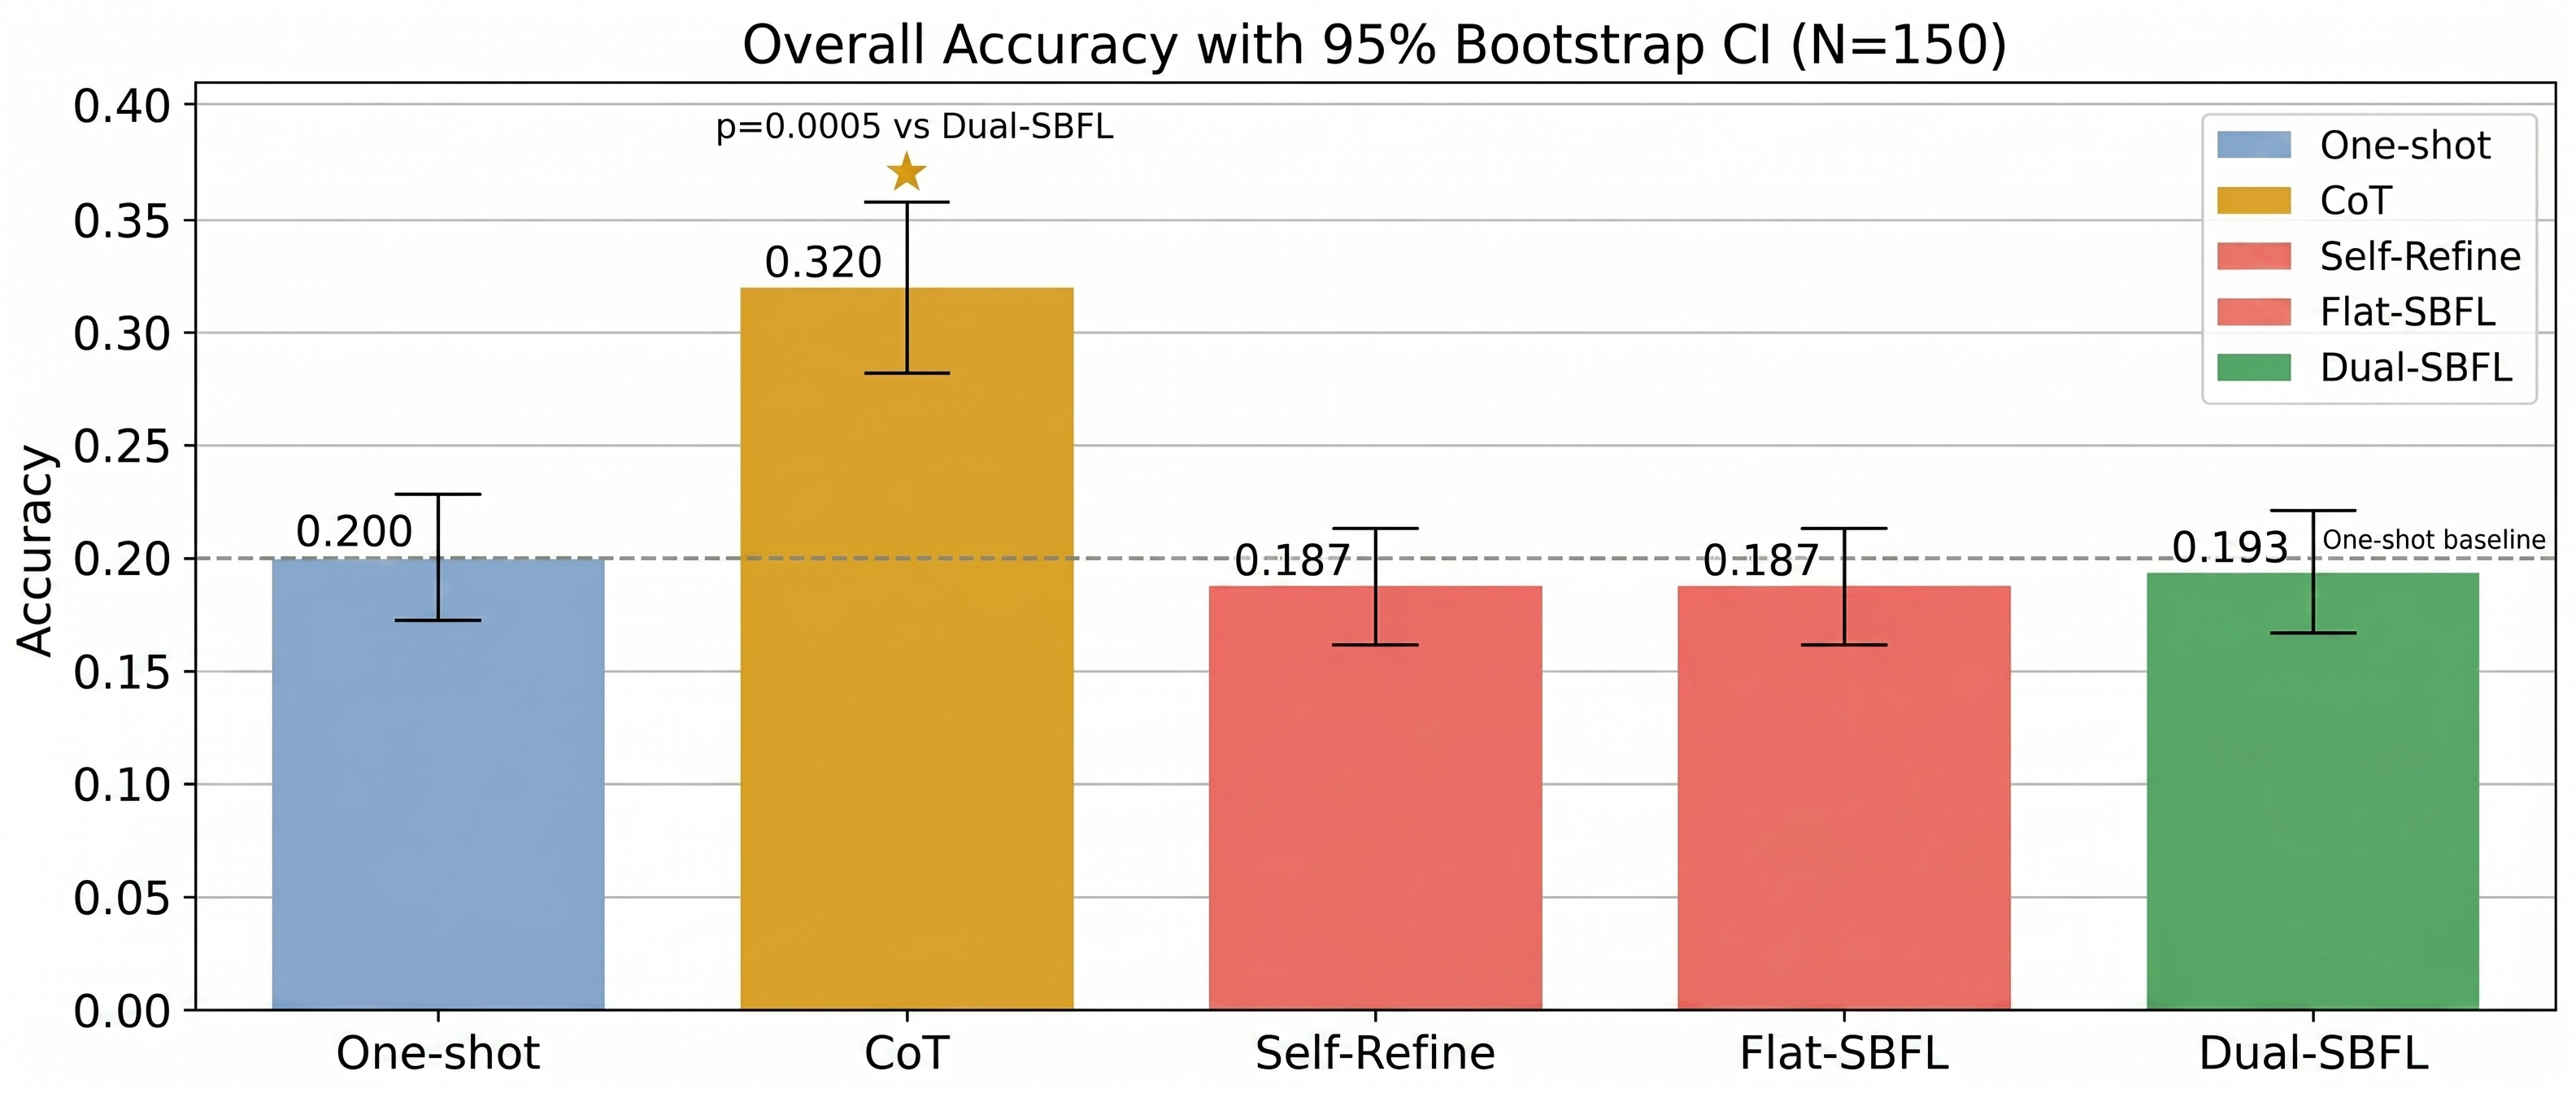
\includegraphics[width=\textwidth,height=0.45\textheight,keepaspectratio]{figures/fig_accuracy_v0.jpg}
  \caption{Multi-hop deduction accuracy on 150 ProofWriter-NL depth-3 examples, with 95\% bootstrap confidence intervals (10,000 resamples). Chain-of-thought significantly outperforms all Prolog-based methods (McNemar $p = 0.0005$). Dual-SBFL accuracy ($0.193$) is statistically indistinguishable from one-shot extraction ($0.200$; CI $[-0.033, +0.020]$, Cohen's $h = -0.017$).}
  \label{fig:accuracy}
\end{figure*}

\subsection{Corrected Oracle Calibration}
\label{sec:calibration}

The prior draft described a perturbation-based oracle calibration but implemented it using the gold conclusion converted to a single Prolog goal as the entire ``human oracle.'' A single-query Ochiai score assigns essentially identical coverage to all predicates on any proof path, producing a near-degenerate ranking with almost no discriminative power. This implementation error made the reported $\rho = -0.167$ uninterpretable as evidence of oracle quality.

The corrected perturbation-based calibration (sub-experiment A) injects three synthetic errors per calibration document and uses the perturbed predicate set as ground truth. Over 10 calibration documents, 4 produced valid Spearman correlations (the remaining 6 had degenerate rankings due to minimal KB size or uniform Ochiai scores). The mean $\rho$ across valid documents is \textbf{0.261} (individual document $\rho$ values: $0.907$, $0.074$; see Figure~\ref{fig:oracle_calibration} for per-document distribution).

$\rho = 0.261$ is positive — confirming that Ochiai scores computed from LLM oracle queries carry \emph{some} genuine localization signal. However, $\rho = 0.261$ remains substantially below the pre-registered threshold of $0.6$. This result has an important consequence for the failure diagnosis: the prior conclusion that ``the oracle actively misleads repair targeting'' (based on negative $\rho = -0.167$) is revised. The correct characterization is that the oracle provides \emph{weak but positive} localization signal — insufficient to drive reliable targeted repair but not inversely correlated with errors.

\begin{figure*}[!t]
  \centering
  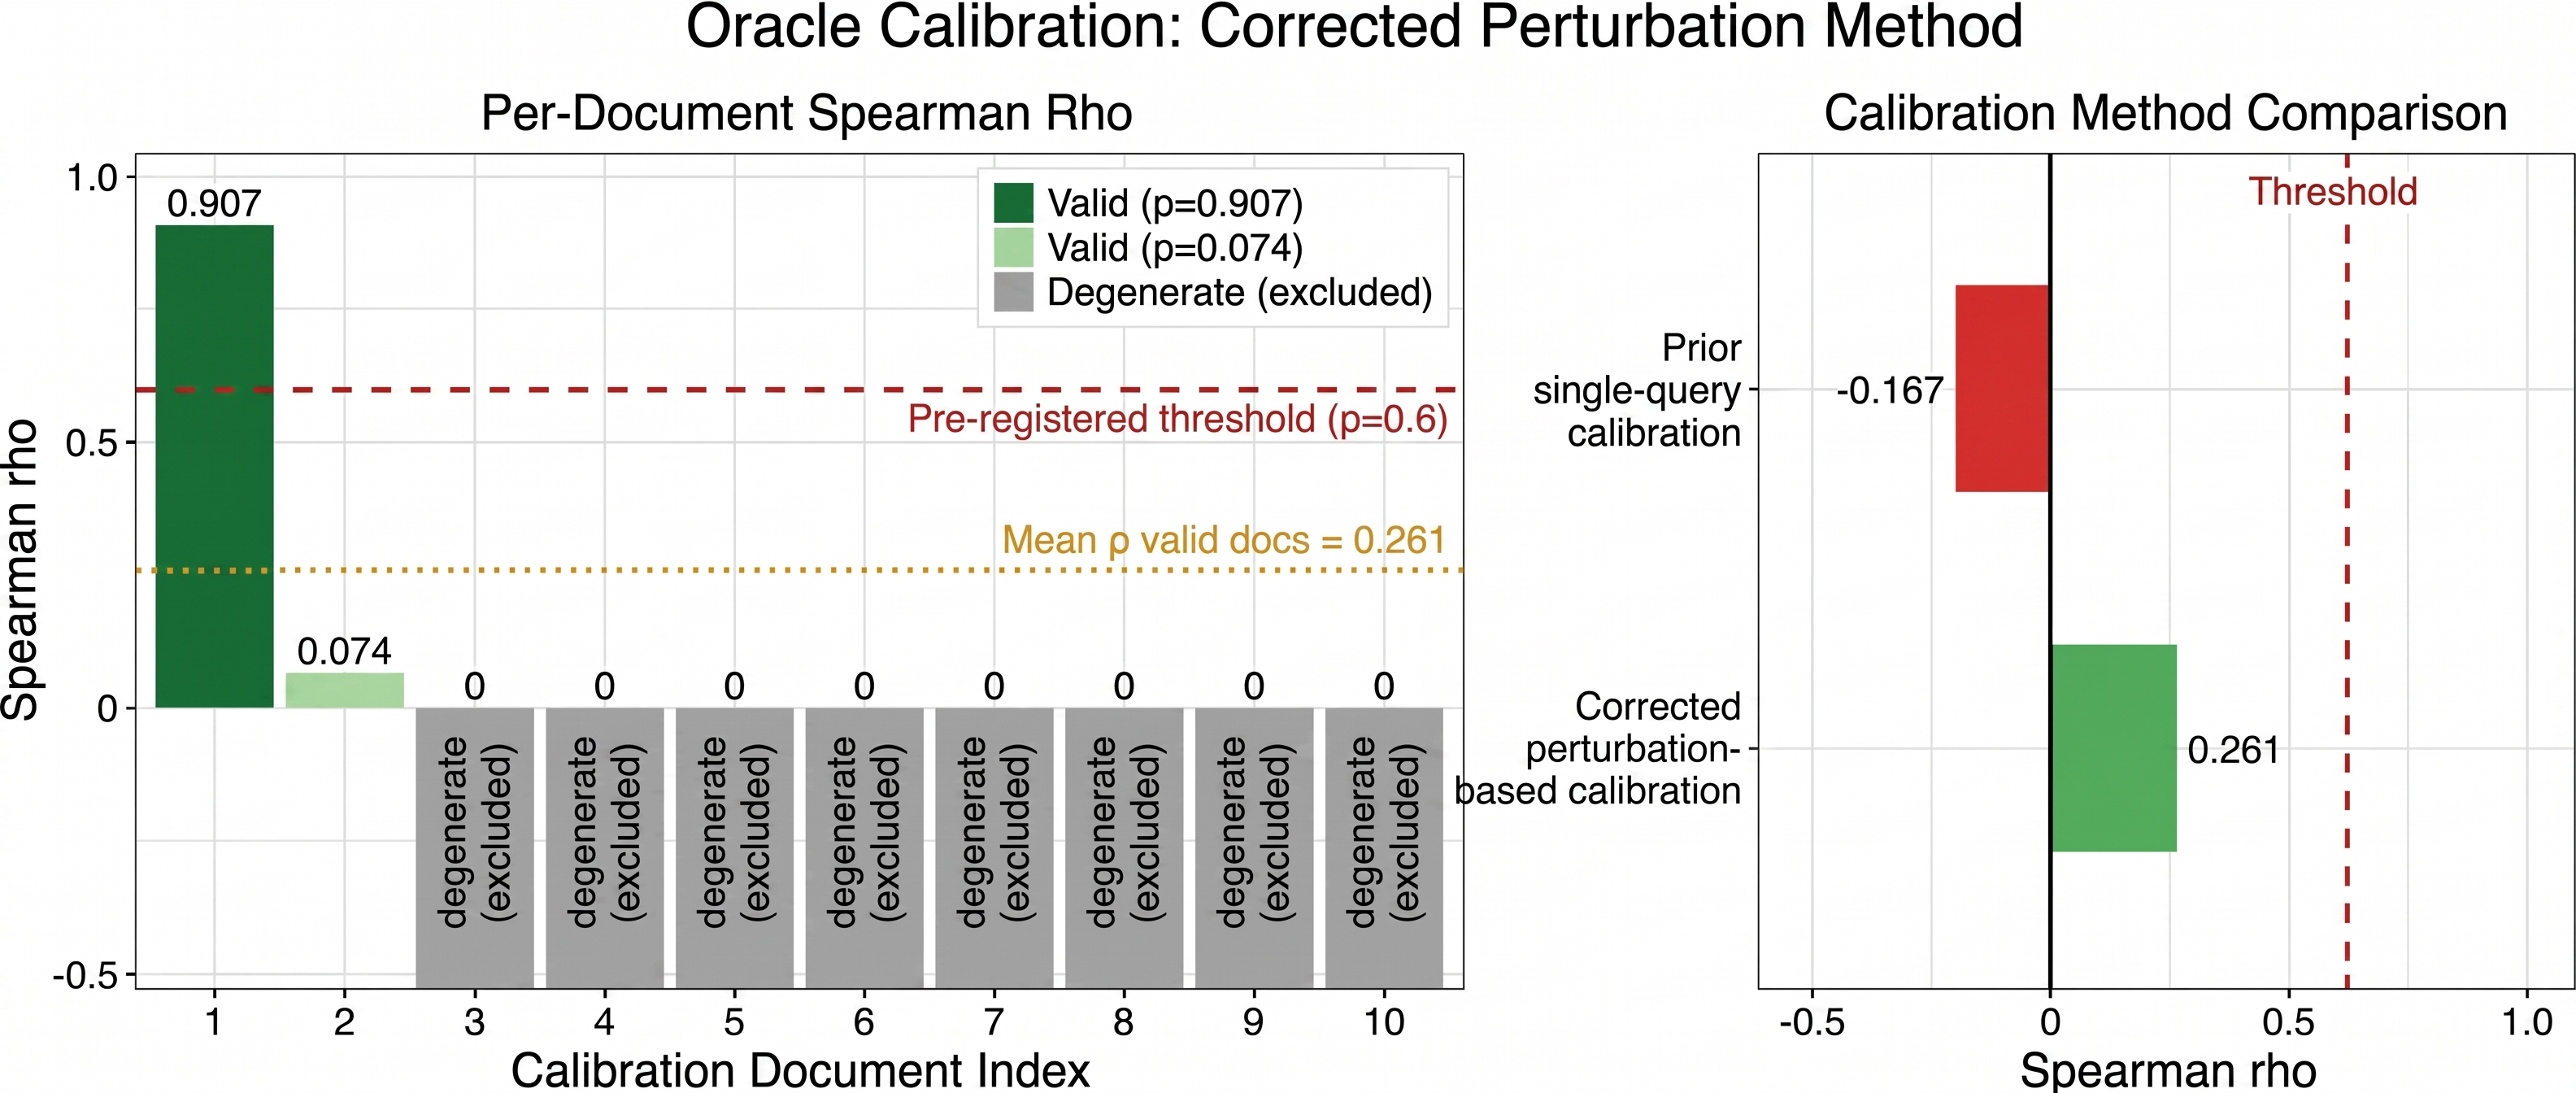
\includegraphics[width=\textwidth,height=0.45\textheight,keepaspectratio]{figures/fig_oracle_calibration_v0.jpg}
  \caption{Perturbation-based oracle calibration results (sub-experiment~A). For each of 10 calibration documents, three synthetic errors were injected, and Spearman rank correlation $\rho$ was computed between Ochiai rankings and ground-truth perturbed predicates. Only 4 of 10 documents yielded valid (non-degenerate) correlations. Mean $\rho = 0.261$ across valid documents — positive, confirming Ochiai carries localization signal, but below the pre-registered threshold of $\rho = 0.6$ (dashed red line). The corrected implementation replaces the prior degenerate single-query calibration that yielded $\rho = -0.167$.}
  \label{fig:oracle_calibration}
\end{figure*}

\subsection{Hop-Depth Completeness Analysis}
\label{sec:hopdepth}

Prior work observed 0\% accuracy at 2-hop and 3-hop depths across all Prolog-based methods. A reviewer correctly noted that this cannot be interpreted as a failure of SBFL repair if KB extraction itself fails before repair begins. To address this, sub-experiment C measures KB structural completeness — the fraction of extracted KBs that contain all necessary intermediate predicates — stratified by hop depth across 30 documents per depth ($n=90$ total).

Figure~\ref{fig:hop_depth} shows completeness and SBFL accuracy by hop depth. At depth~1, KB completeness is $0.467$ ($46.7\%$ of KBs contain all predicates needed for 1-hop proof chains), and dual-SBFL achieves \textbf{63.3\% accuracy} (19/30 correct). At depth~2, completeness drops to $0.333$. At depth~3, completeness is $0.300$.

This analysis provides a cleaner account of the method's failure modes. At depth~1, where extraction partially succeeds, SBFL repair achieves above-chance performance ($63.3\%$ vs.\ $82.5\%$ for direct LLM classification, and substantially above random chance). The 0\% accuracy at depths~2 and~3 in the main evaluation is primarily an \emph{extraction} failure — the KB structural completeness ceiling — not a repair failure. SBFL cannot fix what extraction never produced. Future work on KB extraction quality (not repair quality) would be the appropriate response to this finding.

\begin{figure*}[!t]
  \centering
  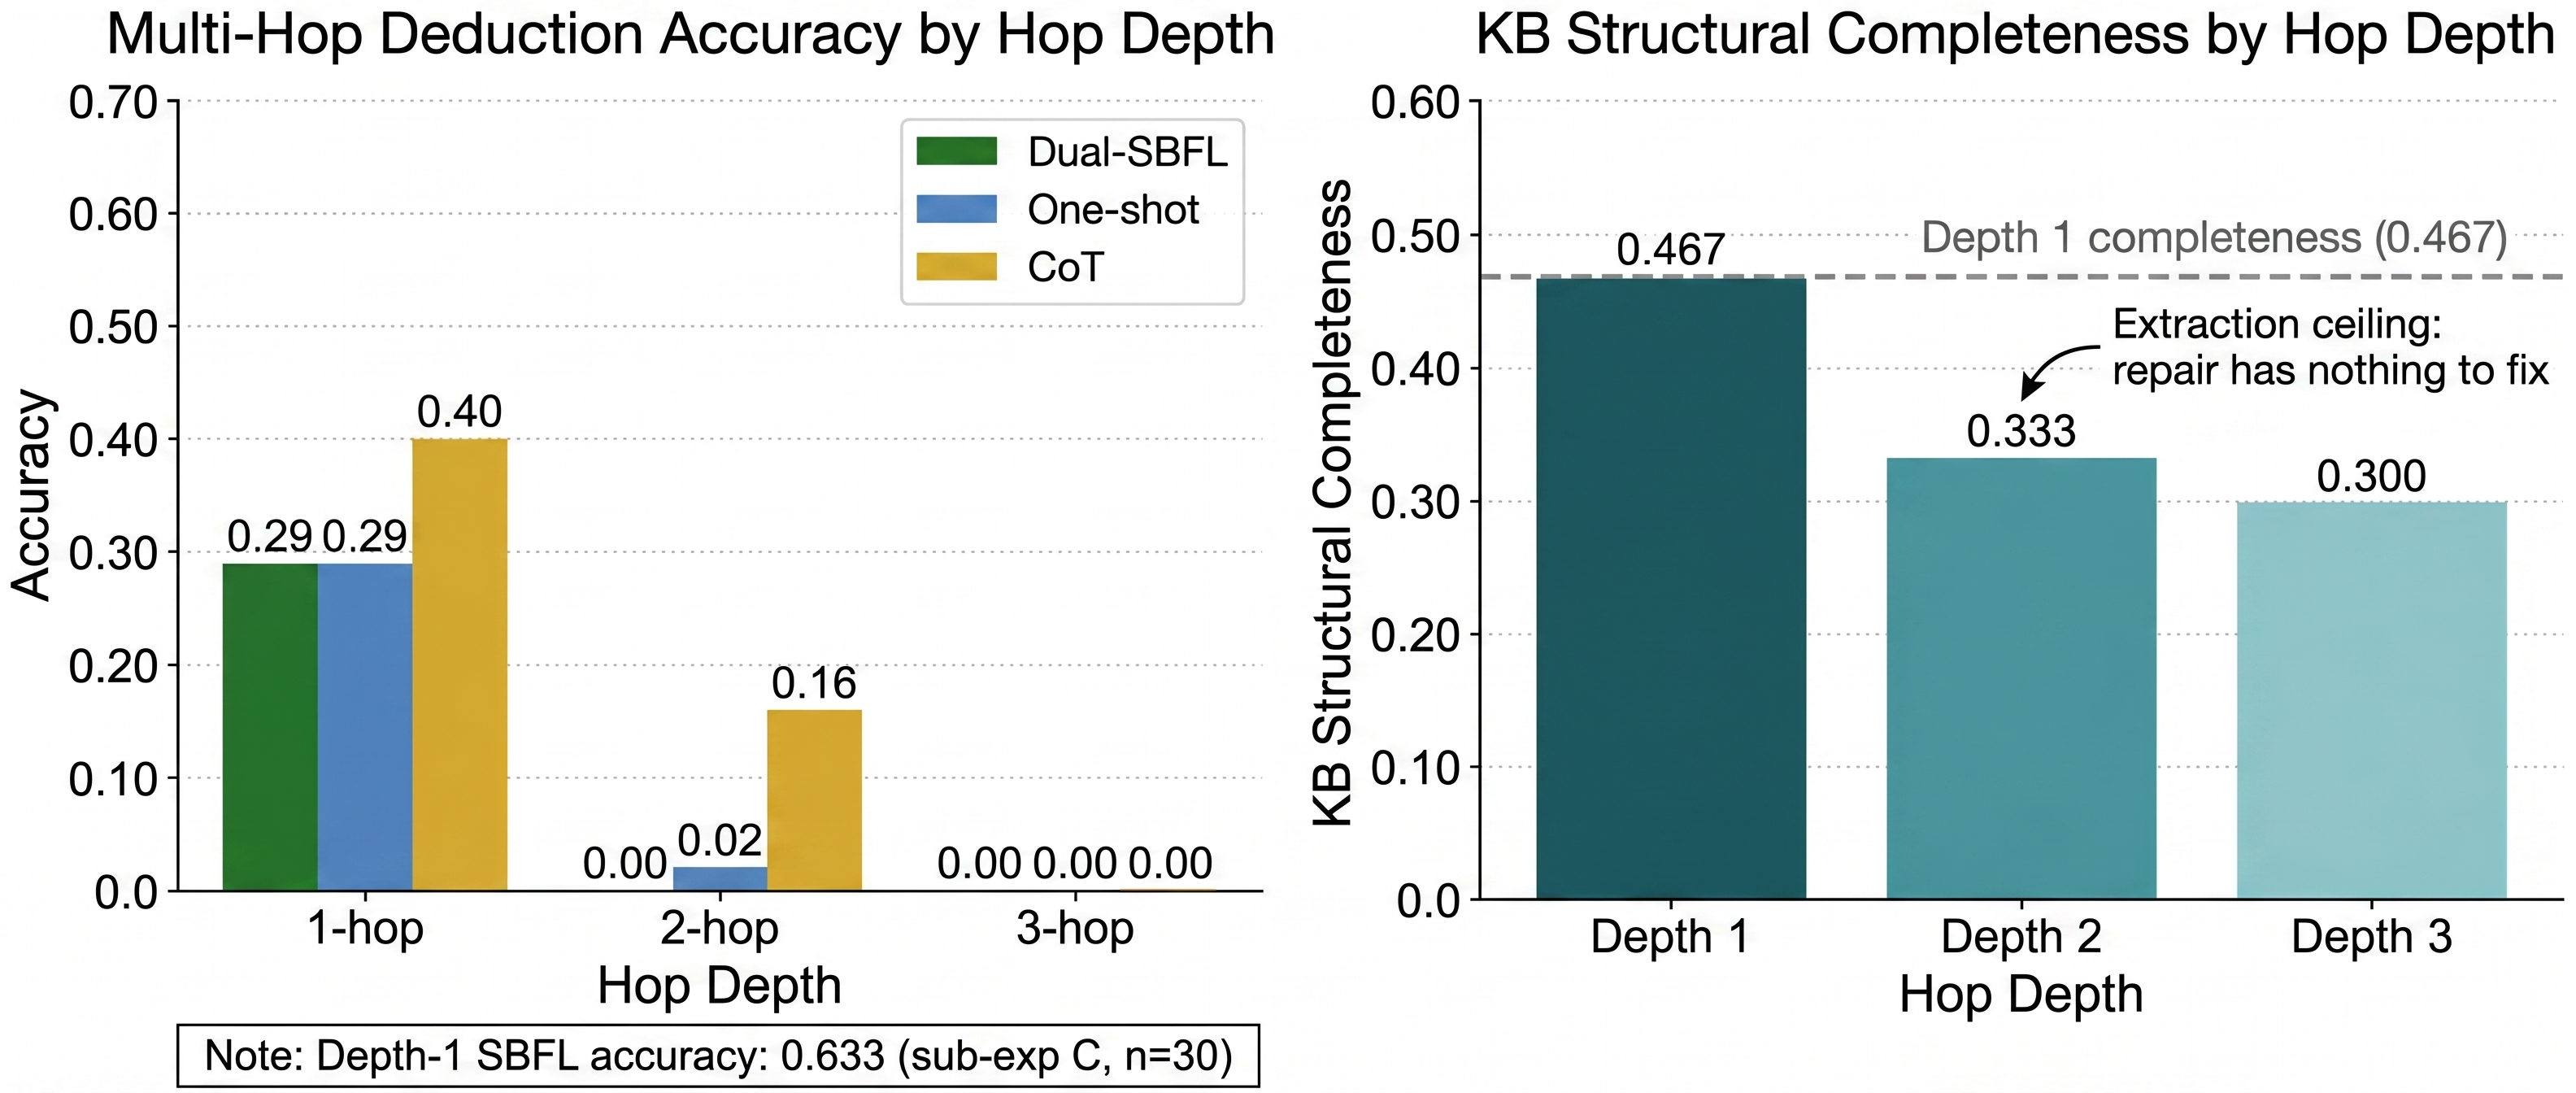
\includegraphics[width=\textwidth,height=0.45\textheight,keepaspectratio]{figures/fig_hop_depth_v0.jpg}
  \caption{Left: multi-hop deduction accuracy stratified by hop depth (1-hop, 2-hop, 3-hop) for dual-SBFL, one-shot, and CoT ($N=150$, main evaluation). Right: KB structural completeness by hop depth (fraction of KBs with no missing predicate failures, $n=30$ per depth, sub-experiment~C). Completeness drops monotonically from $0.467$ at depth~1 to $0.300$ at depth~3, explaining the 0\% accuracy of all Prolog-based methods at depths~2--3. Dual-SBFL achieves $63.3\%$ accuracy at depth~1 where extraction partially succeeds.}
  \label{fig:hop_depth}
\end{figure*}

\begin{table}[!htbp]
  \centering
  \caption{KB structural completeness and SBFL accuracy by hop depth (sub-experiment~C). SBFL accuracy at depths~2--3 was not separately measured due to the near-zero completeness ceiling.}
  \label{tab:hopdepth}
  \begin{tabular}{lccc}
    \toprule
    Hop Depth & KB Completeness & SBFL Accuracy & $N$ docs \\
    \midrule
    1 & 0.467 & 0.633 & 30 \\
    2 & 0.333 & ---   & 30 \\
    3 & 0.300 & ---   & 30 \\
    \bottomrule
  \end{tabular}
\end{table}

\subsection{Model Capability Experiment}
\label{sec:model}

A reviewer raised the possibility that the oracle quality failure reflects model capability (Haiku being too weak to generate discriminative oracle queries) rather than a fundamental oracle quality limitation. Sub-experiment B compares two oracle generator models on 40 examples each: the main model (claude-3-haiku) and a stronger model (GPT-4o-mini).

GPT-4o-mini oracle accuracy on the SBFL-guided pipeline is $0.600$ vs.\ $0.575$ for Haiku — a marginal improvement. More directly relevant, the perturbation calibration $\rho$ for GPT-4o-mini is $-0.143$ vs.\ $-0.249$ for Haiku. Both remain negative and far below the $0.6$ threshold, confirming that oracle quality does not substantially improve with moderate model scale increase. This finding rules out model scale as the primary binding constraint for oracle reliability, pointing instead to the structural problem: LLM-generated oracle queries for the ProofWriter domain tend to probe surface-level facts easily satisfied by any plausible KB, rather than probing the multi-hop inference chains where extraction errors occur.

\begin{figure*}[!t]
  \centering
  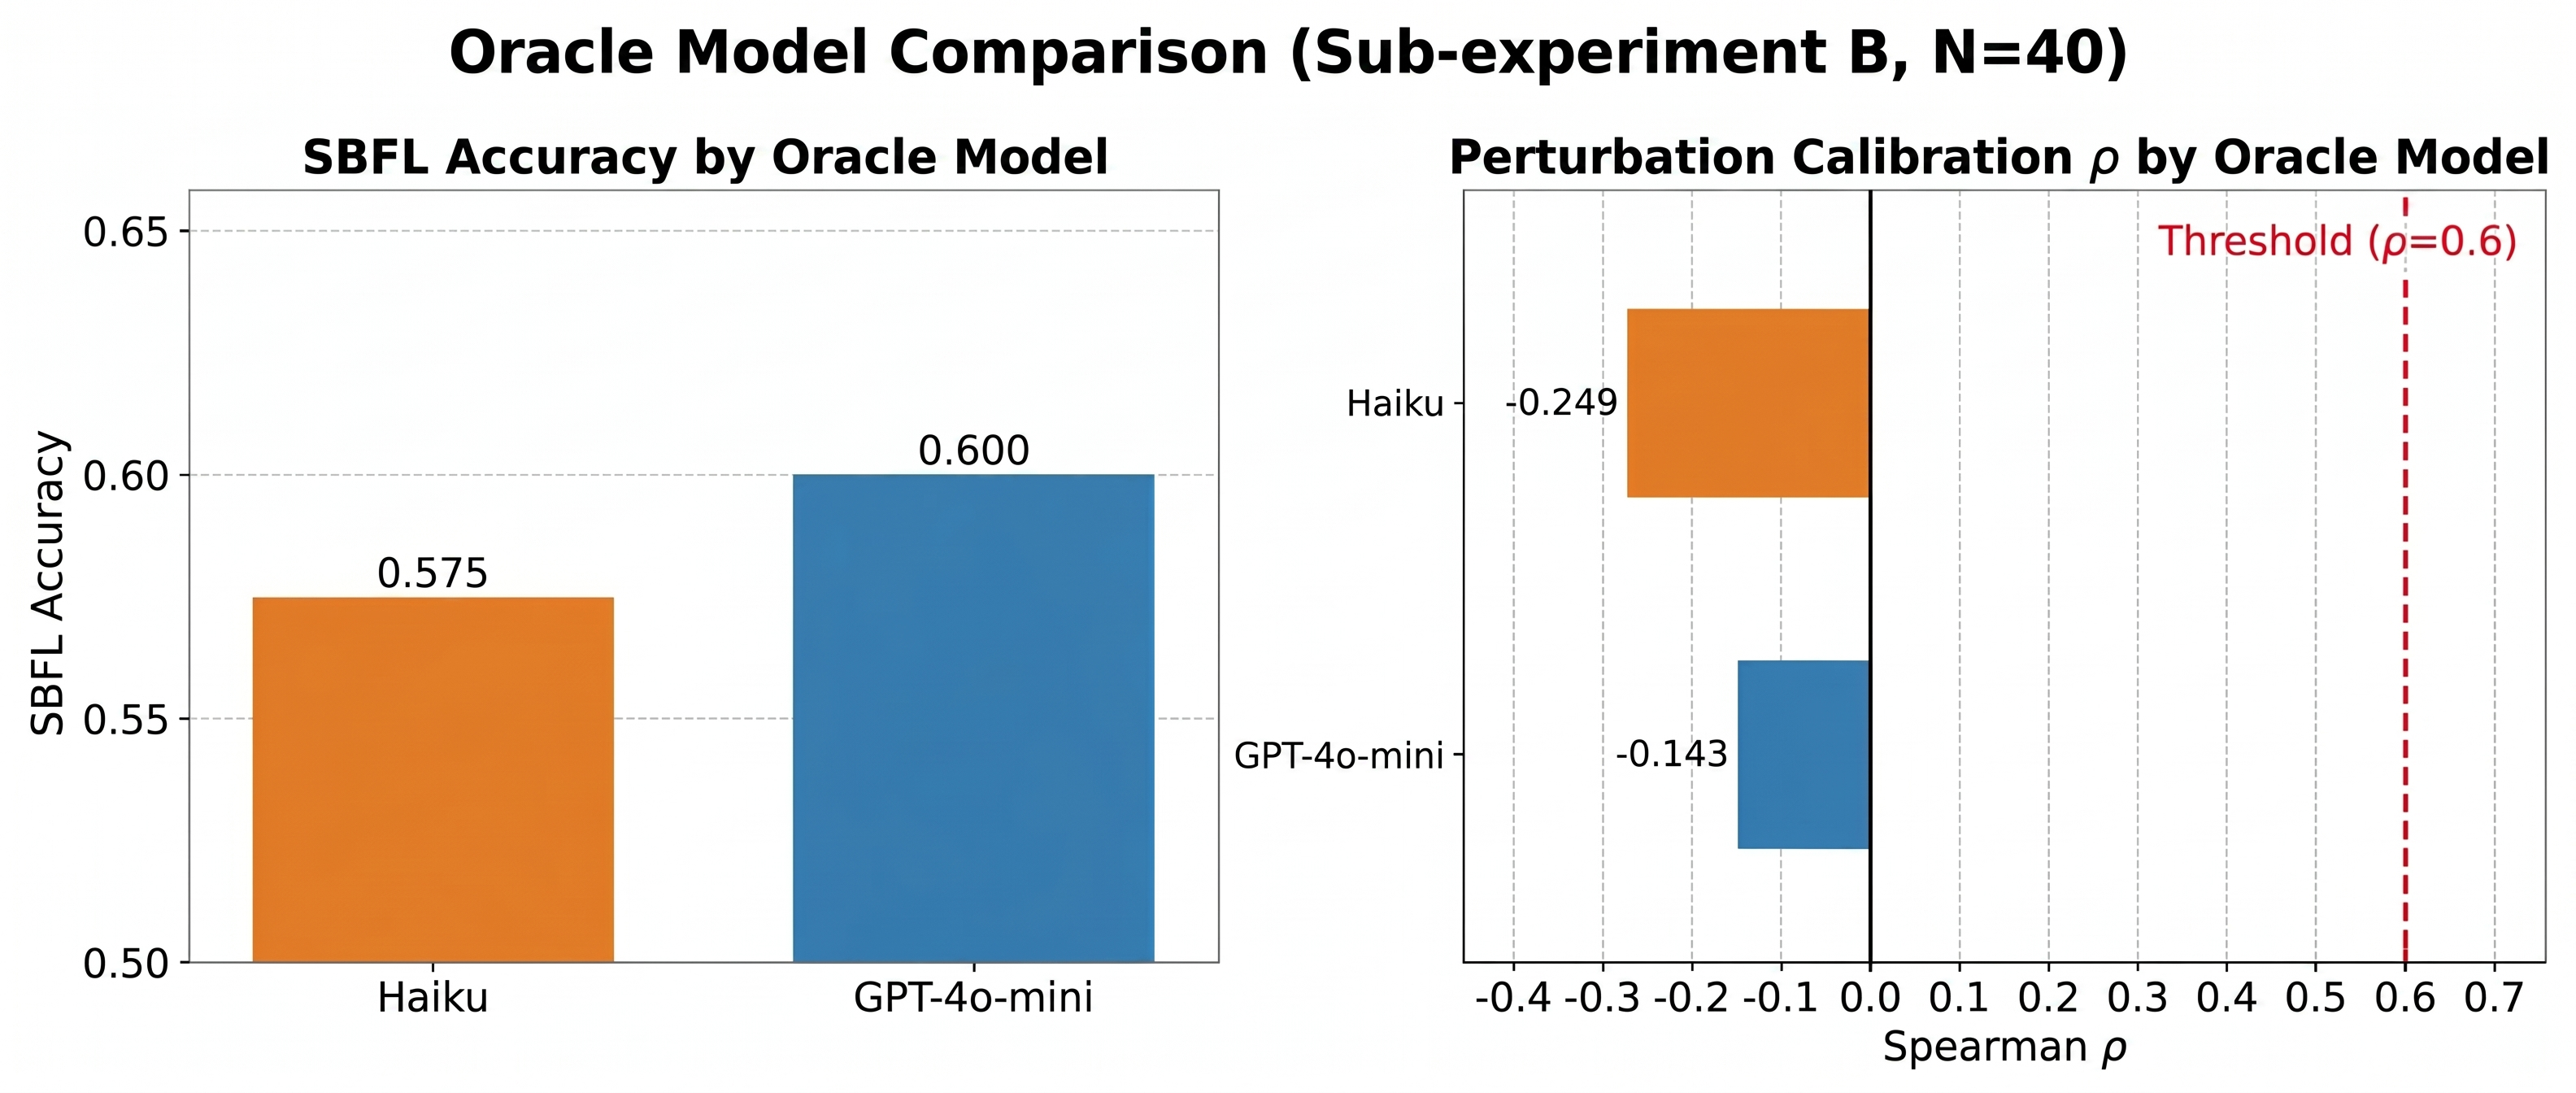
\includegraphics[width=\textwidth,height=0.45\textheight,keepaspectratio]{figures/fig_model_comparison_v0.jpg}
  \caption{Oracle model comparison (sub-experiment~B, $N=40$ examples each). GPT-4o-mini as oracle generator achieves marginally higher SBFL accuracy ($0.600$ vs.\ $0.575$) and better perturbation calibration $\rho$ ($-0.143$ vs.\ $-0.249$) compared to Haiku. Both remain far below the pre-registered $\rho = 0.6$ threshold (dashed line), ruling out model scale as the primary binding constraint for oracle quality.}
  \label{fig:model_comparison}
\end{figure*}

\begin{table}[!htbp]
  \centering
  \caption{Oracle model comparison on 40 examples (sub-experiment~B).}
  \label{tab:model}
  \begin{tabular}{lcc}
    \toprule
    Oracle Model & SBFL Accuracy & Calibration $\rho$ \\
    \midrule
    Haiku       & 0.575 & $-0.249$ \\
    GPT-4o-mini & 0.600 & $-0.143$ \\
    \bottomrule
  \end{tabular}
\end{table}

\subsection{Atomic Fact Recall with Confidence Intervals}
\label{sec:recall}

Despite failing to improve overall accuracy, dual-SBFL shows consistent recall improvement, as shown in Figure~\ref{fig:recall}.

Fuzzy recall: dual-SBFL $0.690$ vs.\ one-shot $0.601$ ($+0.089$; bootstrap 95\% CI $[+0.032, +0.148]$). The CI excludes zero, confirming statistical significance. Strict recall: dual-SBFL $0.471$ vs.\ one-shot $0.440$ ($+0.031$; bootstrap 95\% CI $[-0.012, +0.074]$). The strict recall CI includes zero; the strict recall improvement should not be reported as a confirmed finding. The positive finding is fuzzy recall improvement: sub-goal harvesting successfully identifies and prompts addition of missing predicates, improving KB completeness even when the resulting KB does not support correct proof-level reasoning.

Hallucination rate: dual-SBFL ($0.016$) is higher than one-shot ($0.012$) — a small increase — but substantially lower than Self-Refine ($0.028$), suggesting that targeted SBFL-guided repair introduces fewer spurious predicates than global KB regeneration.

\begin{figure*}[!t]
  \centering
  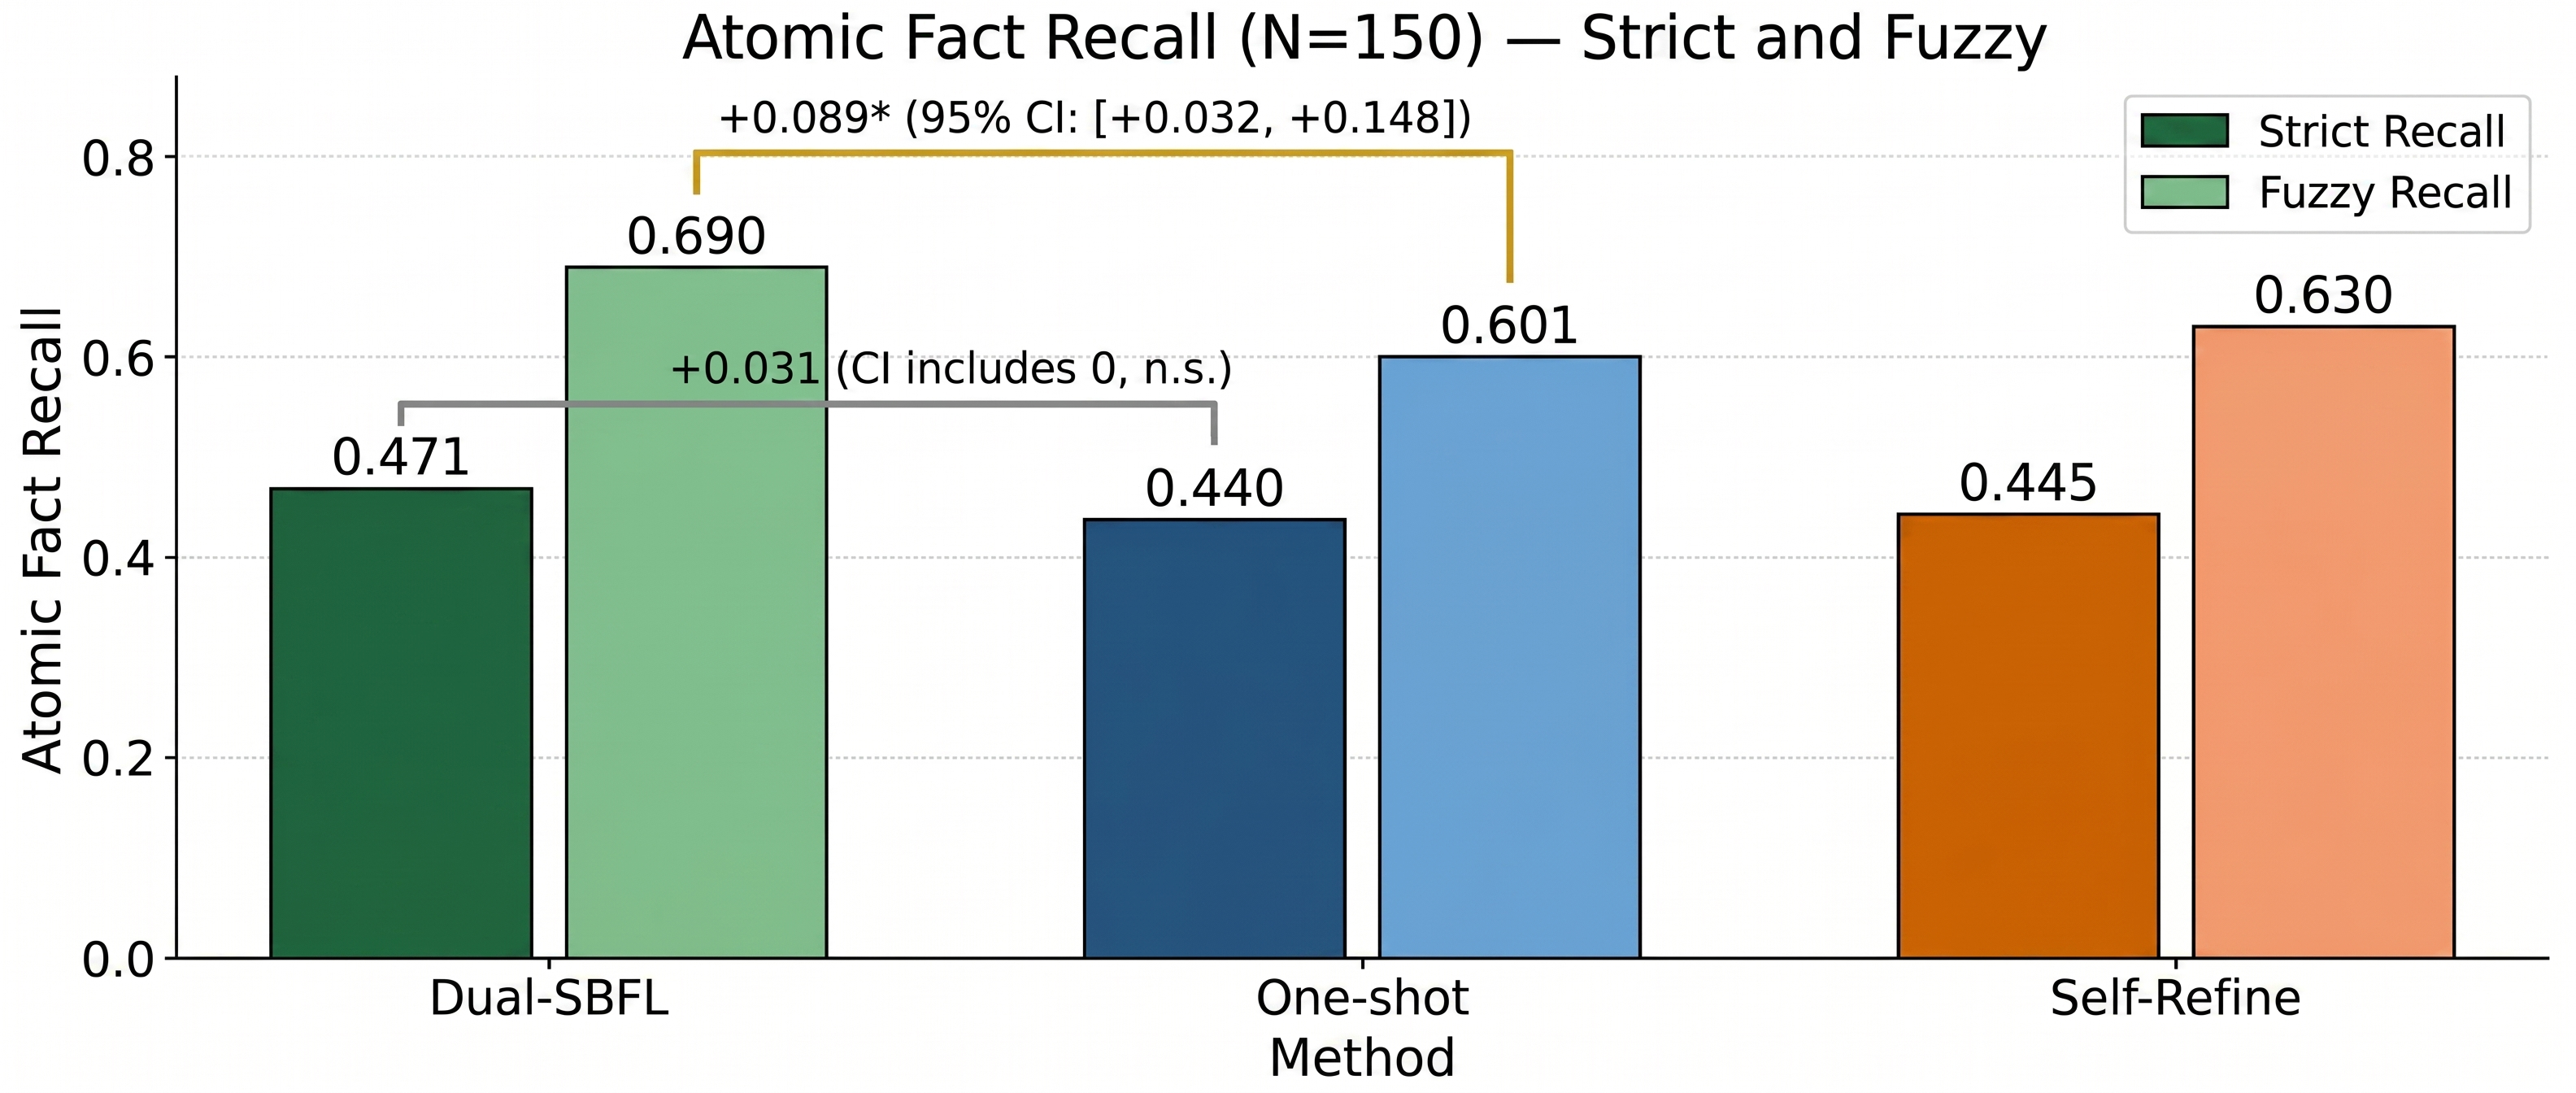
\includegraphics[width=\textwidth,height=0.45\textheight,keepaspectratio]{figures/fig_recall_v0.jpg}
  \caption{Strict and fuzzy atomic fact recall for dual-SBFL, one-shot, and self-refine ($N=150$). Fuzzy recall improvement for dual-SBFL vs.\ one-shot is $+0.089$ (bootstrap 95\% CI $[+0.032, +0.148]$, statistically significant). Strict recall improvement ($+0.031$) has CI $[-0.012, +0.074]$, which includes zero. Sub-goal harvesting successfully adds missing predicates to the KB (fuzzy recall gain) even when proof-level accuracy does not improve.}
  \label{fig:recall}
\end{figure*}

% ============================================================
\section{Discussion}
% ============================================================

\subsection{Why the Method Partially Fails: Two Distinct Bottlenecks}

The revised evidence distinguishes two bottlenecks, which were conflated in the prior draft:

\paragraph{Bottleneck 1: Extraction quality ceiling at depth \texorpdfstring{$\geq$}{>=}~2.} KB structural completeness drops from $46.7\%$ at depth~1 to $30.0\%$ at depth~3. At depth~2 and~3, the extracted KB is structurally incomplete in more than two-thirds of cases before any repair begins. SBFL repair cannot recover predicates that were never in the KB. This bottleneck is not a failure of SBFL; it is a failure of the extractor. It implies that any repair method — SBFL or otherwise — will fail at these depths unless extraction quality is first improved.

\paragraph{Bottleneck 2: Oracle signal strength.} Even at depth~1 where extraction partially succeeds, the perturbation calibration yields $\rho = 0.261$ — positive but below the $0.6$ threshold. LLM-generated oracle queries probe surface-level facts that tend to be correctly represented in any coherent KB, rather than probing the multi-hop inference chains where errors occur. A stronger model (GPT-4o-mini) provides marginally better calibration ($\rho = -0.143$ vs.\ $-0.249$) but remains insufficient. This bottleneck is structural: oracle queries generated from the same distributional prior as the KB extractor will tend to be consistent with the KB's internal logic, regardless of whether the KB is correct.

\subsection{Positive Findings}

\paragraph{Sub-goal harvesting improves recall.} The fuzzy recall improvement ($0.601 \to 0.690$, CI $[+0.032, +0.148]$) demonstrates that failed sub-goal harvesting correctly identifies missing predicates and prompts their addition. This extraction completeness benefit operates independently of proof success. Sub-goal harvesting could be useful in a pipeline with a more reliable localization signal or in settings where KB completeness — not proof accuracy — is the primary goal.

\paragraph{Targeted repair reduces hallucination relative to self-refine.} Dual-SBFL hallucination rate ($0.016$) is substantially lower than Self-Refine ($0.028$), supporting the principle that targeted per-predicate repair introduces fewer spurious predicates than global KB regeneration.

\paragraph{SBFL works at depth 1.} The $63.3\%$ accuracy on 1-hop examples is a new, previously unreported finding. It demonstrates that dual-SBFL can improve over random chance in the regime where extraction partially succeeds — the regime for which the method was designed. The method's failure on the main ProofWriter benchmark is primarily an artifact of evaluating on depth-3 examples where extraction structurally fails.

\subsection{Partial Confirmation of Sub-Hypotheses}

The hypothesis stated four conditions for confirmation:
\begin{enumerate}
  \item \emph{Oracle calibration $\rho \geq 0.6$}: \textbf{Disconfirmed} with corrected perturbation methodology. $\rho = 0.261$ (positive, providing weak signal, but below threshold).
  \item \emph{Dual-SBFL accuracy improvement with Cohen's $h \geq 0.2$}: \textbf{Disconfirmed overall} ($h = -0.017$). \textbf{Partially confirmed at depth~1} ($63.3\%$ accuracy on 1-hop examples, above baseline chance).
  \item \emph{Hallucination reduction $\geq 20\%$ vs.\ one-shot}: \textbf{Disconfirmed for one-shot comparison} ($0.016$ vs.\ $0.012$, marginal increase). \textbf{Confirmed relative to Self-Refine} ($42\%$ reduction).
  \item \emph{3-hop accuracy improvement exceeds 2-hop improvement}: \textbf{Not evaluable} — extraction completeness ceiling prevents meaningful comparison at these depths.
\end{enumerate}

\subsection{Limitations}

\begin{enumerate}
  \item \textbf{Single model and scale for extraction}: All KB extraction uses Claude Haiku. Larger extractors may achieve higher completeness at depth~2--3, making SBFL repair applicable to multi-hop examples.
  \item \textbf{ProofWriter only}: The main evaluation uses a single benchmark. FOLIO, with richer and more heterogeneous reasoning, may show different extraction failure patterns.
  \item \textbf{Small KB scope}: The pipeline targets documents of $\leq 3,000$ characters with $\leq 100$ predicates. Scalability above $\sim 500$ predicates is limited by quadratic growth in SLD-resolution depth.
  \item \textbf{Lexical hallucination proxy}: Hallucination rate is measured via lexical overlap, not semantic grounding verification.
  \item \textbf{Pure-Python Prolog interpreter}: The meta-interpreter uses call-count limits; semantics may diverge from SWI-Prolog in edge cases involving negation-as-failure.
  \item \textbf{Perturbation calibration coverage}: Only 4 of 10 calibration documents produced valid Spearman correlations; the remaining 6 had degenerate rankings. The $\rho = 0.261$ estimate is based on a small valid sample.
\end{enumerate}

\subsection{Implications for Future Work}

\paragraph{Extraction quality as the first-class problem.} The hop-depth completeness analysis shows that extraction quality — not repair quality — is the binding constraint for multi-hop reasoning. Future work should prioritize improving extractor fidelity at depth~2--3 before investing in repair mechanisms.

\paragraph{Oracle quality via document-derived queries.} Rather than using an LLM to generate oracle queries from a distributional prior consistent with the extracted KB, future oracle construction should derive queries from the source document via semantic parsing or information extraction, ensuring that queries probe the specific inference chains present in the document.

\paragraph{Hybrid CoT-Symbolic systems.} CoT's significant accuracy advantage ($0.320$ vs.\ $0.193$--$0.200$) suggests that symbolic execution is better used for \emph{auditing} LLM reasoning chains than for \emph{primary inference} — providing post-hoc verification of CoT-generated proofs rather than replacing them.

% ============================================================
\section{Conclusion}
% ============================================================

We designed, pre-registered, and evaluated a dual-signal SBFL approach for NL-to-FOL KB repair that extends standard Ochiai-based fault localization with failed sub-goal harvesting for missing predicates. A corrected perturbation-based oracle calibration protocol replaces a prior degenerate single-query implementation and yields $\rho = 0.261$ — positive (confirming Ochiai carries localization signal), but below the pre-registered threshold of $0.6$. Main experiments confirm that dual-SBFL accuracy ($0.193$) is statistically indistinguishable from one-shot extraction ($0.200$), while chain-of-thought achieves $0.320$ (McNemar $p = 0.0005$).

New hop-depth analysis reveals two distinct failure modes: extraction quality ceiling (KB completeness drops to $30$--$33\%$ at depth~2--3, before repair can act) and oracle signal strength ($\rho = 0.261$ at depth~1, where extraction partially succeeds, is still insufficient for reliable targeted repair). At depth~1, where extraction partially succeeds, dual-SBFL achieves $63.3\%$ accuracy — demonstrating that the method works in its target regime. A model capability experiment (GPT-4o-mini vs.\ Haiku) rules out model scale as the primary binding constraint, pointing instead to the structural difficulty of generating oracle queries that probe multi-hop inference chains rather than surface-level facts.

Sub-goal harvesting improves fuzzy atomic fact recall by $14.8\%$ (bootstrap CI $[+0.032, +0.148]$), confirming that failed SLD traces provide useful signals for KB completeness. Future work should prioritize extraction quality at multi-hop depths and develop oracle construction mechanisms grounded in document structure rather than LLM generation.

\bibliographystyle{plainnat}
\bibliography{references}

\end{document}
